\documentclass[30pt,landscape]{foils}
\usepackage[german,english]{babel}  % Sprachunterst�tzung
\usepackage[latin1]{inputenc}       % wir benutzen Latin1-Zeichen
\usepackage{ifvtex}
\usepackage{ifpdf}
% Wenn wir vtex benutzen, erzeugen wir wom�glich auch pdf...
\ifvtexpdf\pdftrue\fi
\ifpdf
\usepackage{pause}               % l�dt auch color
\usepackage{background}
\usepackage{graphicx}            % Pdf-Ausgabe f�r Bilder
\usepackage{geometry}
\usepackage{hyperref}
\else
\usepackage[dvipdfm]{pause}      % l�dt auch color
\usepackage[dvipdfm]{background}
\usepackage[dvips]{graphicx}
\usepackage[dvips]{geometry}
\usepackage[dvipdfm]{hyperref}
%% Die nachstehende Definition ist nur notwendig, weil wir Varianten
%% derselben Graphik als .mps und .eps vorhalten. Die .mps-Variante ist
%% geeignet f�r pdflatex und dvipdfm, die .eps-Variante f�r vlatex und
%% pdflatex. Daher m�ssen wir hier f�r dvipdfm die Bevorzugung von .mps
%% erzwingen.
%% matrixb?.eps ist aus matrixb?.fig mit der Option -p2 von fig2dev
%% entstanden. matrixb?.mps entsteht bei normaler Umsetzung (siehe Manual). 
\DeclareGraphicsExtensions{.jpg,.jpeg,.pdf,.png,.mps,.eps,.ps}
\fi
\usepackage{pp4slide}
\geometry{headsep=3ex,hscale=0.9}
\hypersetup{pdftitle={pdftexdemo},
  pdfsubject={Eine Demonstration von LaTeX und Acrobat},
  pdfauthor={Klaus Guntermann, FG Systemprogrammierung, TU Darmstadt
  <guntermann@iti.informatik.tu-darmstadt.de>},
  pdfkeywords={pdftex, acrobat},
  pdfpagemode={FullScreen},
  colorlinks={true},
  linkcolor={red}
  }
\begin{document}
{\Large\normalcolor\bf
  \LaTeX{} und Acrobat Reader\\
  \null\hfill f�r Pr�sentationen\break}

\noindent
F�r Pr�sentationen sind Spezialprogramme wie PowerPoint oder
MagicPoint bisher stark vertreten.\pause\\
Aber mit etwas Nachhilfe kann man auch mit \TeX/\LaTeX{}
Pr�sentationen erstellen, die sich sehen lassen k�nnen.\pause\\
Dieses Beispieldokument zeigt, wie man den Acrobat Reader im
Ganzseitenmodus benutzen kann.\pause

{\tiny
Mit Return/Enter/PageDown geht es weiter\hfill\pauselevel{=1}}

\foilhead{Was kann man damit machen?}
\begin{itemize}
\item Ganz normale Aufz�hlungen\pause
  \begin{itemize}
  \item nat�rlich auch geschachtelt\pause
  \item und mit unterschiedlichen Symbolen
    \begin{itemize}
    \item auch in dieser Tiefe\pause
    \end{itemize}
  \item und hier weiter\pause
  \end{itemize}
\item und der Schluss
\end{itemize}

\foilhead{Wer mag, kann auch Hintergr�nde definieren}
\definecolor{bgblue}{rgb}{0.04,0.39,0.53}
\vpagecolor{bgblue}
\begin{itemize}
\item Einfarbigen Hintergrund hatten wir ja schon.
\item Diese Seite hat einen leicht verlaufenden Hintergrund. (Bei
  Bildschirmen, die nicht im TrueColor-Modus arbeiten, kann das
  seltsam aussehen.)
\item �berg�nge k�nnen auch anders als auf einen Schlag erfolgen...
\end{itemize}

\foilhead{Noch mehr "`Hintergr�ndiges"'}
\hypersetup{pdfpagetransition=Dissolve}
\definecolor{bgmag}{rgb}{0.7,0.39,0.7}
\hpagecolor{bgmag}
...wenn man solche Spielereien mag.
\begin{itemize}
\item Hintergr�nde k�nnen auch horizontal verlaufen.\pause
\item Weitere Beispiele mit krasseren Farb�nderungen ersparen wir uns aber.
\end{itemize}

\foilhead[-1cm]{Was geht besser als bei PowerPoint etc.?}
\hypersetup{pdfpagetransition=R}
\vpagecolor{bgblue}
Im wissenschaftlichen Bereich ben�tigt man bei Pr�sentationen
auch die M�glichkeit, Formeln zu benutzen.\pause\\
Der Formelsatz bei den weit verbreiteten Pr�sentations\-werkzeugen l�sst
jedoch zu w�nschen �brig.\pause\\
Wenn man seine Texte mit \LaTeX{} formatiert, macht so etwas
aber kein Problem:
$$
  \sum_{i=0}^\infty a_i\cdot x^i
$$

\foilhead[-4.1cm]{Man kann auch Formeln entwickeln...}
\begin{eqnarray*}
H(s) &=& \int_{-\infty}^{+\infty} h(t) e^{2\pi ist} dt\pause\\
     &=& \int_{-\infty}^{+\infty} \left\{\int_{-\infty}^{+\infty}
         f(\xi) \cdot g(t - \xi) d \xi \right\} e^{2 \pi ist} dt\pause\\
     &=& \int_{- \infty}^{+ \infty} f(\xi) \left\{ \int_{- \infty}^{+
         \infty} g(t - \xi) \cdot e^{2\pi is(t - \xi)} dt\right\}
         \cdot e^{2\pi is \xi} d \xi\pause\\
     &=& \int_{- \infty}^{+ \infty} f(\xi) G(s) e^{2\pi is \xi} d \xi\pause\\
     &=& G(s) \cdot \int_{- \infty}^{+ \infty} f(\xi)e^{2\pi is \xi} d
         \xi\pause = G(s) \cdot F(s)
\end{eqnarray*}

\foilhead[-2cm]{Verweise}

Es ist m�glich, innerhalb einer Pr�sentation auch zu
\hyperlink{Ende}{springen}, wenn man auf einen anderen Sachverhalt zu
sprechen kommen will. Sei es als Vorgriff oder als R�ckw�rtsverweis.
Wenn Sie oben das Wort "`springen"' anklicken, gelangen Sie auf eine
andere Seite dieses Dokuments. Finden Sie dort das Wort "`Zur�ck"' und
klicken Sie es an, damit Sie wieder hier ankommen.\pause\\
Wenn Ihr Acrobat Reader entsprechend eingestellt ist, k�nnen Sie auch
einen Web-Browser aktivieren. Probieren Sie, auf die WWW-Seite von
PPower4 zu gelangen, indem Sie
\href{http://www-sp.iti.informatik.tu-darmstadt.de/software/ppower4/}{hier}
anklicken.

\foilhead[-2cm]{Bilder}
\vpagecolor{bgmag}
Nat�rlich kann man auch Bilder einbinden und der Reihe nach zeigen\pause,
auch gemischt mit Text.
  \begin{center}
  %% vlatex will include the .eps variants, pdflatex the .mps version...
  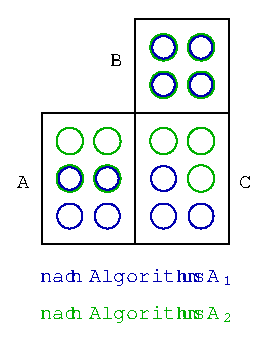
\includegraphics[scale=1.6]{matrixb1}
  \pause\qquad\qquad
  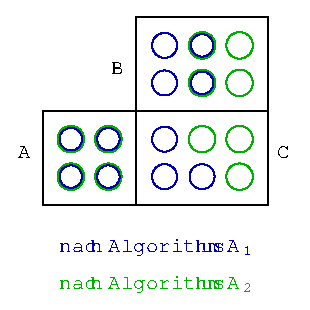
\includegraphics[scale=1.6]{matrixb2}
  \end{center}
{\small Diese Bilder wurden mit XFig erstellt und �ber MetaPost-Export
  skalierbar eingebunden.}

\foilhead[-3cm]{Das Ende}
\vpagecolor{bgblue}

Vielen Dank f�r das Interesse an dieser kurzen Demonstration.

Mehr Informationen finden Sie im 
\href{http://www-sp.iti.informatik.tu-darmstadt.de/software/ppower4/bericht.pdf}%
{Bericht} �ber PPower4, dem Programm mit dem dieses Dokument bearbeitet wurde.
Beachten Sie aber, dass dieser Bericht nur die anf�ngliche Entwicklung
beschreibt und nicht den aktuellen Stand.
\hypertarget{Ende}{}
\vfill

{\small
Mit \texttt{Esc} verl�sst man den FullScreen-Modus von Acrobat-Reader.\\
�ber das View-Men� k�nnen Sie diesen Modus ggf.\ wieder einstellen.\\
\hbox to \textwidth{\hfill \Acrobatmenu{GoBack}{Zur�ck} zur
  vorher angezeigten Seite.}\par}
%\enlargethispage{1cm}
\end{document}
